\documentclass[ngerman,a4paper,order=firstname]{../../texmf/tex/latex/mathscript/mathscript}
\usepackage{../../texmf/tex/latex/mathoperators/mathoperators}

\title{\textbf{Stochastik SS 2019}}
\author{Dozent: Prof. Dr. \person{Anita Behme}}

\begin{document}
\pagenumbering{roman}
\pagestyle{plain}

\maketitle

\hypertarget{tocpage}{}
\tableofcontents
\bookmark[dest=tocpage,level=1]{Inhaltsverzeichnis}

\pagebreak
\pagenumbering{arabic}
\pagestyle{fancy}

\chapter*{Vorwort}
Wir freuen uns, dass du unser Skript für die Vorlesung \textit{Geometrie} bei Prof. Dr. Arno Fehm im WS2018/19 gefunden hast. Da du ja offensichtlich seit einem Jahr Mathematik studierst, kannst du dich glücklich schätzen zu dem einen Drittel zu gehören, dass nicht bis zum zweiten Semester abgebrochen hat.

Wenn du schon das Vorwort zu \textit{Lineare Algebra und analytische Geometrie 1+2} gelesen hast, weißt du sicherlich, dass Prof. Fehm ein Freud der Algebra ist.\footnote{In Zukunft wird sich Prof. Fehm richtig freuen dürfen, denn im Zuge einer neuen Studienordnung, die am 1.4.2019 in Kraft tritt, kommt so gut wie keine Geometrie im \textit{Bachelor Mathematik} vor.} Auf die Frage eines Kommilitonen, wo in seinem Inhaltsverzeichnis (Gruppen, Ringe, Körper) die Geometrie vorkomme, antwortete er:
\begin{quote}
	\textit{Die Frage ist nicht, wieso wir in dieser Vorlesung Algebra statt Geometrie machen, sondern warum hier seit 20 Jahren Geometrie unterrichtet wird.}
\end{quote}

Wie auch im letzten Vorwort können wir dir nur empfehlen die Vorlesung immer zu besuchen, denn dieses Skript ist kein Ersatz dafür. Es soll aber ein Ersatz für deine unleserlichen und (hoffentlich nicht) unvollständigen Mitschriften sein und damit die Prüfungsvorbereitung einfacher machen. Im Gegensatz zu letztem Semester veröffentlicht Prof. Fehm auf seiner Homepage (\url{http://www.math.tu-dresden.de/~afehm/lehre.html}) kein vollständiges Skript mehr, sondern nur noch eine Zusammenfassung.

Der Quelltext dieses Skriptes ist bei Github (\url{https://github.com/henrydatei/TUD_MATH_BA}) gehostet; du kannst ihn dir herunterladen, anschauen, verändern, neu kompilieren, ... Auch wenn wir das Skript immer wieder durchlesen und Fehler beheben, können wir leider keine Garantie auf Richtigkeit geben. Wenn du Fehler finden solltest, wären wir froh, wenn du ein neues Issue auf Github erstellst und dort beschreibst, was falsch ist. Damit wird vielen (und besonders nachfolgenden) Studenten geholfen.

Und jetzt viel Spaß bei \textit{Geometrie}!

\begin{flushright}
	Henry, Pascal und Daniel
\end{flushright}

\chapter*{Was ist Stochastik?}

Altgriechisch Stochastikos ($\sigma \tau o \chi \alpha \sigma \tau \iota \kappa$\`{o}$ \zeta$) und bedeutet sinngemäß ``scharfsinning in Vermuten''.\\
Fragestellung insbesondere aus Glückspiel, Versicherung-/Finanzmathematik, überall da wo Zufall/ Risiko / Chance auftauchen.\\
Was ist Stochastik?
\begin{itemize}
	\item Beschreibt zufällige Phänomene in einer exakten Spache!\\
	Beispiel: ``Beim Würfeln erscheint jedes sechste Mal (im Schnitt) eine 6.'' $\longrightarrow$ Gesetz der großen Zahlen ($\nearrow$ später) %TODO set ref
	\item Lässt sich mathematische Stochastik in zwei Teilgebiete unterteilen\\
	Wahrscheinlichkeitstheorie (W-Theorie) \& Statistik
	\begin{itemize}
		\item \textit{W-Theorie}: Beschreibt und untersucht konkret gegebene Zufallssituationen.
		\item \textit{Statistik}: Zieht Schlussfolgerungen aus Beobachtungen.
	\end{itemize}
	Statistik benötigt Modelle der W-Theorie und W-Theorie benötigt die Bestätigung der Modelle durch Statistik.
\end{itemize}
In diesem Semester konzentrieren wir uns nur auf die Wahrscheinlichkeitstheorie!
% Grundbegriffe der WTheorie
\chapter{Grundbegriffe der Wahrscheinlichkeitstheorie}

\section{Wahrscheinlichkeitsräume}

\subsection*{Ergebnisraum}

Welche der möglichen Ausgänge eines zufälligen Geschehens interessieren uns?\\
Würfeln? Augenzahl, nicht die Lage und die Fallhöhe

\begin{definition}[Ergebnisraum]
	Die Menge der relevanten Ergebnisse eines Zufallsgeschehens nennen wir \begriff{Ergebnisraum} und bezeichnen diesen mit $\Omega$.
\end{definition}

\begin{*example}
	\begin{itemize}
		\item Würfeln: $\Omega = \{1,2, \dots, 6\}$
		\item Wartezeiten: $\Omega = \real_{+} = [0, \infty)$ (überabzählbar!)
	\end{itemize}
\end{*example}

\subsection*{Ereignisse}

Oft interessieren wir uns gar nicht für das konkrete Ergenis des Zufallsexperiments, sondern nur für das Eintreten gewisser Ereignisse.
\begin{*example}
	\begin{itemize}
		\item Würfeln: Zahl ist $\ge 3$
		\item Wartezeit: Wartezeit $\le 5$ Minuten
	\end{itemize}
\end{*example}

$\longrightarrow$ Teilmenge des Ereignisraums, also Element der Potenzmenge $\mathscr{P}(\Omega)$, denen eine Wahrscheinlichkeit zugeordnet werden kann, d.h. welche \begriff{messbar} (mb) sind.

\begin{definition}[Ereignisraum, messbarer Raum]
	Sei $\Omega \neq \emptyset$ ein Ergebnisraum und $\mathscr{F}$ eine $\sigma$-Algebra auf $\Omega$, d.h. eine Familie von Teilmenge von $\Omega$, sodass
	\begin{enumerate}
		\item $\Omega \in \mathscr{F}$
		\item $A \in \mathscr{F} \Rightarrow A^C \in \mathscr{F}$
		\item $A_1, A_2, \dots \in \mathscr{F} \Rightarrow \bigcup_{i \ge 1} \in \mathscr{F}$
	\end{enumerate}
	Dann heißt $(\Omega, \mathscr{F})$ \begriff{Ereignisraum} bzw. \begriff{messbarer Raum}.
\end{definition}

\subsection*{Wahrscheinlichkeiten}

Ordne Ereignissen Wahrscheinlichkeiten zu mittels der Abbildung

\begin{align}
	\mathbb{P}: \mathscr{F} \to [0,1]\notag
\end{align}

sodass

\begin{align}
	\text{Normierung } \mathbb{P}(\Omega) = 1 \tag{N}\label{eq_norm}\\
	\sigma\text{-Additivität für paarweise disjunkte Ereignisse} \tag{A}\label{eq_additive}\\
	A_1, A_2, \dots \in \mathscr{F} \Rightarrow \mathbb{P}(\bigcup_{i \ge 1} A_i) = \sum_{1 \ge 1} \mathbb{P}(A_i)\notag
\end{align}

\cref{eq_norm}, \cref{eq_additive} und die Nichtnegativität von $\mathbb{P}$ werden als \begriff{\person{Kolmogorov}sche Axiome} bezeichnet (nach Kolomogorov: Grundbegriffe der Wahrscheinlichkeitstheorie, 1933)

\begin{definition}[Wahrscheinlichkeitsmaß, Wahrscheinlichkeitsverteilung]
	Sei $(\Omega, \mathscr{F})$ ein Ereignisraum und $\mathbb{P}: \mathscr{F} \to [0,1]$ eine Abbildung mit Eigenschaften \cref{eq_norm} und \cref{eq_additive}. Dann heißt $\mathbb{P}$ \begriff{Wahrscheinlichkeitsmaß} oder auch \begriff{Wahrscheinlichkeitsverteilung}.
\end{definition}

Aus der Definition folgen direkt:

\begin{proposition}[Rechenregeln für W-Maße]
	\proplbl{1_4}
	Sei $\mathbb{P}$ ein W-Maß, Ereignisse $(\Omega, \mathscr{F}), A, B, A_1, A_2, \dots \in \mathscr{F}$. Dann gelten:
	\begin{enumerate}
		\item $\mathbb{P}(\emptyset) = 0$
		\item Monotonie: $A \subseteq B \Rightarrow \mathbb{P}(A) \le \mathbb{P}(B)$
		\item endliche $\sigma$-Additivität: $\mathbb{P}(A\cup B) + \mathbb{P}(A\cap B) = \mathbb{P}(A) + \mathbb{P}(B)$ und insbesondere $\mathbb{P}(A) + \mathbb{P}(A^C) = 1$
		\item $\sigma$-Subadditivität:
		\begin{align}
			\mathbb{P}\left(\bigcup_{i \ge 1} A_i\right) \le \sum_{1 \ge 1} \mathbb{P}(A_i)\notag
		\end{align}
		\item $\sigma$-Stetigkeit: Wenn $A_n \uparrow A$ (d.h. $A_1 \subseteq A_2 \subseteq \cdots$ und $A = \bigcup_{i=1}^{\infty} (A_i)$) oder $A_n \downarrow A$, so gilt:
		\begin{align}
			\mathbb{P}(A_n) \longrightarrow \mathbb{P}(A), n \to \infty \notag
		\end{align}
	\end{enumerate}
\end{proposition}

\begin{proof}
	In der Vorlesung wurde nur auf Schillings MINT Vorlesung verwiesen. Der folgende Beweis wurde ergänzt.\\
	Beweise erst folgende Aussage: $A\cap B = \emptyset \Longrightarrow \probp(A \uplus B) = \probp(A) + \probp(B)$.\\
	Es kann $\sigma$-Additivität verwendet werden, indem ``fehlende'' Mengen durch $\emptyset$ ergänzt werden:
	\begin{align}
		\probp(A \uplus B) = \probp(A \uplus B \uplus \emptyset \uplus \emptyset \dots) = \probp(A) + \probp(B) + \probp(\emptyset) + \dots = \probp(A) + \probp(B),\notag
	\end{align}
	wobei Maßeigenschaften verwendet wurden.
	\begin{enumerate}
		\item Definition des Maßes.
		\item Da $A \subseteq B$ ist auch $B = A \uplus (B \setminus A) = A \uplus (B \setminus (A \cap B))$. Wende wieder Aussage von oben an, damit folgt
		\begin{align}
			\probp(B) = \probp(A \uplus (B \setminus A)) = \probp(A) + \probp(B \setminus A) \ge \probp(A) \label{eq_1_1_4}\tag{*}
		\end{align}
		\item Zerlege $A \cup B$ geschickt, dann sieht man mit oben gezeigter Aussage und \cref{eq_1_1_4}
		\begin{align}
			\probp(A \cup B) + \probp(A \cap B) &= \probp(A \uplus (B \setminus (A \cap B)) + \probp(A \cap B)\notag \\
			&= \probp(A) + \probp(B \setminus (A \cap B)) + \probp(A \cap B)\notag\\
			&= \probp(A)+\probp(B).\notag	
		\end{align}
		Im letzten Schritt wurde \cref{eq_1_1_4} verwendet.
		\item Folgt aus endlicher $\sigma$-Additivität, da $\probp\left(\bigcap_{i\ge 1} A_i \right) \ge 0$.
		\item Definiere $F_1 := A_1, F_2 := A_2 \setminus A_1, \dots, F_{i+1} := A_{i+1}\setminus A_n$. Die $F_i$ Mengen sind paarweise disjunkt und damit folgt für $m \to \infty$
		\begin{align}
			A_m = \biguplus_{i=1}^{m} F_i \Rightarrow A = \biguplus_{i=1}^{\infty} F_i = \biguplus_{i=1}^{\infty} A_i\notag
		\end{align}
		und
		\begin{align}
			\probp(A) = \probp\left( \biguplus_{i=1}^{\infty} F_i \right) = \sum_{i=1}^{\infty} \probp(F_i) = \lim\lim_{m \to \infty} \probp\left( \biguplus_{i=1}^{m} F_i \right) = \lim\lim_{m\to \infty} \probp(A_m). \notag
		\end{align}
	\end{enumerate}
\end{proof}

\begin{example}
	Für ein beliebigen Ereignisraum $(\Omega, \mathscr{F})$ ($\Omega \neq \emptyset$) und eine beliebiges Element $\xi \in \Omega$ definiere
	\begin{align}
		\delta_{\xi}(A := \begin{cases}
		1 & \xi \in A \\
		0 & \text{ sonst}
		\end{cases}\notag
	\end{align}
	eine (degeneriertes) W-Maß auf $(\Omega, \mathscr{F})$, welches wir als \begriff{\person{Dirac}-Maß} oder \begriff{\person{Dirac}-Verteilung} bezeichnen.
\end{example}

\begin{example}
	Würfeln mit fairem, $6$-(gleich)seitigem Würfel mit Ergebnismenge $\Omega=\{1, \dots, 6\}$ und Ereignisraum $\mathscr{F} = \mathscr{P}(\Omega)$ setzen wir als Symmetriegründen
	\begin{align}
		\mathbb{P}(A) = \frac{\# A}{6}.\notag
	\end{align}
	(Wobei $\# A$ oder auch $\vert A \vert$ die Kardinalität von $A$ ist.) Das definiert ein W-Maß.
\end{example}

\begin{example}
	\proplbl{1_1_7}
	Wartezeit an der Bushaltestelle mit Ergebnisraum $\Omega = \real_{+}$ und Ereignisraum \person{Borel}sche $\sigma$-Algebra $\mathscr{B}(\real_{+}) = \mathscr{F}$. Eine mögliches W-Maß können wir dann durch
	\begin{align}
	\mathbb{P}(A) = \int_{A} \lambda e^{-\lambda x} \diff x\notag %TODO set a mathoperator for dx!!!
	\end{align}
	für einen Parameter $\lambda > 0$ festlegen. (Offenbar gilt $\mathbb{P}(\Omega) = 1$ und die $\sigma$-Additivität aufgrund der Additivität des Integrals.) Wir bezeichnen diese Maß als \begriff{Exponentialverteilung}. (Warum gerade dieses Maß für Wartezeiten gut geeignet ist $\nearrow$ später) %TODO add later a ref!!!
\end{example}

%%%%%%%%%%%%%%%%%%%%%%%%%%%%%%%% 2nd Lecture %%%%%%%%%%%%%%%%%%%%%%%%%%%%%%%%%%%%%%%%%%%%

\begin{proposition}[Konstruktion von WMaßen durch Dichten]
	\proplbl{1_8}
	Sei $(\Omega, \mathscr{F})$ ein Eriegnisraum.
	\begin{itemize}
		\item $\Omega$ abzählbar, $\mathscr{F} = \mathscr{P}(\Omega)$: Sei $\rho = (\rho(\omega))_{\omega \in \Omega}$ eine Folge in $[0,1]$ in $\sum_{\omega \in \Omega} \rho(\omega) = 1$, dann definiert
		\begin{align}
			\probp(A) = \sum_{\omega \in \Omega} \rho(\omega), A \in \mathscr{F} \notag
		\end{align}
		ein (diskretes) WMaß $\probp$ auf $(\Omega, \mathscr{F})$. $\rho$ wird als \begriff{Zähldichte} bezeichnet.
		\item Umgekehrt definiert jedes WMaß $\probp$ auf $(\Omega, \mathscr{F})$ definiert Folge $\rho(\omega) = \probp(\set{\omega}), \omega \in \Omega$ eine Folge $\rho$ mit den obigen Eigenschaften.
		\item $\Omega \subset \Rn, \mathscr{F} = \mathscr{B}(\Omega)$: Sei $\rho: \Omega \to [0, \infty)$ eine Funktion, sodass
		\begin{enumerate}
			\item $\int_{\Omega} \rho(x)\diff x = 1$
			\item $\set{x \in \Omega \colon f(x) \le c} \in \mathscr{B}(\Omega)$ für alle $c > 0$ 
		\end{enumerate}
		dann definiert $\rho$ ein WMaß $\probp$ auf $(\Omega, \mathscr{F})$ durch 
		\begin{align}
		\probp(A) = \int_{A} \rho(x) \diff x = \int_{A} \rho \diff \lambda, \quad A \in \mathscr{B}(\Omega).\notag
		\end{align}
		Das Integral interpretieren wir stets als Lebesgue-Integral bzw. Lebesgue-Maß $\lambda$.
		$\rho$ bezeichnet wir als \begriff{Dichte}, \begriff{Dichtefunktion}/\begriff{Wahrscheinlichkeitsdichte} von $\probp$ und nennen ein solches $\probp$ \begriff{(absolut)stetig (bzgl. denn Lebesgue-Maß)}.
	\end{itemize}
\end{proposition}

\begin{proof}
	\begin{itemize}
		\item Der diskrete Fall ist klar.
		\item Im stetigen Fall folgt die Bahuptung aus den bekannten Eigenschaften des Lebesgue-Integrals ($\nearrow$ Schilling MINT, Lemma 8.9)
	\end{itemize}
\end{proof}

\begin{*remark}
	\begin{itemize}
		\item Die Eineindeutige Beziehung zwischen Dichte und WMaß überträgt sich nicht auf den stetigen Fall.
		\begin{itemize}
			\item Nicht jedes WMaß auf $(\Omega, \mathscr{B}(\Omega)), \Omega \subset \Rn$ besitzt eine Dichte.
			\item Zwei Dichtefunktionen definieren dasselbe WMaß, wenn sie sich nur auf einer Menge von Lebesgue-Maß $0$ unterscheiden.
		\end{itemize}
		\item Jede auf $\Omega \subset \Rn$ definiert Dichtefunktion $\rho$ lässt sich auf ganz $\Rn$ fortsetzen durch $\rho(x) = 0, x \not\in \Omega$. Das erzeugte WMaß auf $(\Rn, \mathscr{B}(\Omega))$ lässt mit den WMaß auf $(\Omega, \mathscr{\Omega})$ identifizieren.
		\item Mittels Dirac-Maß $\delta_{x}$ können auch jedes diskrete WMaß auf $\Omega \subset \Rn$ als WMaß auf $\Rn, \mathscr{B}(\Rn)$ intepretieren
		\begin{align}
			\probp(A) = \sum_{\omega \in A} \rho(\omega) = \int_{A} \diff \left( \sum_{\omega \in \Omega} \rho(\omega)\delta_{\omega} \right)\notag
		\end{align}
		stetige und diskrete WMaße lassen sich kombiniere z.B.
		\begin{align}
			\probp(A) = \frac{1}{2} \delta_{0} + \frac{1}{2} \int_{A}\indi_{[0,1]}(x)\diff x, A \in \mathscr{B}(\R)\notag
		\end{align}
		ein WMaß auf $(\R, \mathscr{B}(\R))$.
	\end{itemize}
\end{*remark}

Abschließend erinnern wir uns an:

\begin{proposition}[Eindeutigkeitssatz für WMaße]
	\proplbl{1_9}
	Sei $(\Omega, \mathscr{F})$ Ereignisraum und $\probp$ ein WMaß auf $(\Omega, \mathscr{F})$. 
	Sei $\mathscr{F} = \omega(\mathscr{G})$ für ein $\cap$-stabiles Erzeugendensystem $\mathscr{G} \subset \mathscr{P}(\Omega)$. 
	Dann ist $\probp$ bereits durch seine Einschränkung $\probp_{\mid \mathscr{G}}$ eindeutig bestimmt.
\end{proposition}

\begin{proof}
	$\nearrow$ Schhiling MINT, Satz 4.5.
\end{proof}

Insbesondere definiert z.B.

\begin{align}
	\probp([0,a]) = \int_{0}^{a} \lambda e^{-\lambda x}\diff x = 1 - e^{-\lambda a}, a > 0 \notag
\end{align}

bereits die Exponentialverteilung aus \propref{1_1_7}.

\begin{definition}[Gleichverteilung]
	Ist $\Omega$ endlich, so heißt das WMaß mit konstanter Zähldichte $\rho(\omega) = \sfrac{1}{\abs{\Omega}}$ die \begriff{(diskrete) Gleichverteilung} auf $\Omega$ und wird mit $U(\Omega)$ notiert (U = Uniform).
	Ist $\Omega \subset \Rn$ eine Borelmenge mit Lebesgue-Maß $0 < \lambda^n(\Omega) < \infty$ so heißt das WMaß auf $(\Omega, \borel(\Omega))$ mit konstanter Dichtefunktion $\rho(x) = \sfrac{1}{\lambda^n(x)}$ die \begriff{(stetige)  Gleichverteilung} auf $\Omega$. 
	Sie wird ebenso mit $U(\Omega)$ notiert.
\end{definition}

\subsection*{WRäume}

\begin{definition}[Wahrscheinlichkeitsraum]
	Ein Tripel $(\Omega, \mathscr{F}, \probp)$ mit $\Omega, \mathscr{F}$ Ereignisraum und $\probp$ WMaß auf $(\Omega, \mathscr{F})$, nennen wir \\ \begriff{Wahrscheinlichkeitsraum}.
\end{definition}

\section{Zufallsvariablen}

Zufallsvariablen dienen dazu von einen gegebenen Ereignisraum $(\Omega, \mathscr{F})$ zu einem Modellausschnitt $\Omega', \mathscr{F}'$ überzugehen. 
Es handelt sich also um Abbildungen $X: \Omega \to \Omega'$.
Damit wir auch jedem Ereignis in $\mathscr{F}'$ eine Wheit zuordnen können, benötigen wir	
\begin{align}
	A' \in \mathscr{F}' \Rightarrow X' A' \in \mathscr{F} \notag		
\end{align}
d.h. $X$ sollte messbar sein.

\begin{definition}[Zufallsvariable]
	Seien $(\Omega, \mathscr{F})$ und $(\Omega', \mathscr{F}')$ Ereignisräume. Dann heißt jede messbare Abbildung
	\begin{align}
		X: \Omega \to \Omega'\notag
	\end{align}
	Zufallsvariable (von $(\Omega, \mathscr{F})$) nach $(\Omega', \sigF')$/ auf $(\Omega', \sigF')$ oder \begriff{Zufallselement}.
\end{definition}

\begin{example}
	\begin{enumerate}
		\item Ist $\Omega$ abzählbar und $\sigF = \pows(\Omega)$, so ist jede Abbildung $X: \Omega \to \Omega'$ messbar und damit eine Zufallsvariable.
		\item Ist $\Omega \subset \Rn$ und $\sigF = \borel(\Omega)$, so ist jede stetige Funktion $X: \Omega \to \R$ messbar und damit eine Zufallsvariable.
	\end{enumerate}
\end{example}

\begin{proposition}
	Sei $(\Omega, \sigF, \probp)$ ein WRaum und $X$ eine Zufallsvariable von $(\Omega, \sigF)$ nach $(\Omega', \sigF')$. Dann definiert
	\begin{align}
		\probp'(A') := \probp\left(X^{-1}(A')\right) = \probp\left(\set{X \in A'}\right), A' \in \sigF'\notag
	\end{align}
	ein WMaß auf $(\Omega', \sigF')$ auf $(\Omega', \sigF')$, welches wir als \begriff{WVerteilung von X unter $\probp$} bezeichnet.
\end{proposition}

\begin{proof}
	Aufgrund der Messbarkeit von $X$ ist die Definition sinnvoll. Zudem gelten
	\begin{align}
		\probp'(\Omega') = \probp(X^{-1}(\Omega')) = \probp(\Omega) = 1\notag
	\end{align}
	und für $A_1', A_2', \dots \in \sigF'$ paarweise disjunkt.
	\begin{align}
		\probp'\left( \bigcup_{i \ge 1} A_i'\right) &= \probp\left(X^{-1}\left( \bigcup_{i \ge 1} A_i' \right)\right) \notag \\
		&= \probp\left( \bigcup_{i \ge 1} X^{-1}(A_i') \right) \notag \\
		&= \sum_{1 \ge 1} \probp(X^{-1}A_i') \notag
	\end{align}
	da auch $X^{-1}A_1', X^{-1}A_2', \dots$ paarweise disjunkt
	\begin{align}
		&= \sum_{1 \ge 1} \probp'(A_i')\notag
	\end{align}
	Also ist $\probp'$ ein WMaß. %TODO put in 1 align to have everything aligned?
\end{proof}

\begin{*remark}
	\begin{itemize}
		\item Aus Gründen der Lesbarkeit schreiben wir in der Folge $\probp(X \in A) = \probp(\set{\omega \colon X(\omega) \in A})$
		\item Ist $X$ die Identität, so fallen die Begriffe WMaß und WVerteilung zusammen.
		\item In der (weiterführenden) Literatur zu WTheorie wird oft auf die Angabe eines zugrundeliegenden WRaumes verzichtet und stattdessen eine ``Zufalsvariable mit Verteilung $\probp$ auf $\Omega$'' eingeführt.
		Gemeint ist (fast) immer $X$ als Identität auf $(\Omega, \sigF, \probp)$ mit $\sigF = \pows(\Omega) / \borel(\Omega)$.
		\item Für die Verteilung von $X$ unter $\probp$ schreibe $\probp_{X}$ und $X \sim \probp_{X}$ für die Tatsache, dass $X$ gemäß $\probp_{X}$ verteilt ist.
	\end{itemize}
\end{*remark}

\begin{definition}[identisch verteilt, reellen Zufallsvariablen]
	Zwei Zufallsvariablen sind \begriff{identisch verteilt}, wenn sie dieselbe Verteilung haben.
	Von besonderen Interesse sind für uns die Zufallsvariablen, die nach $(\R, \borel(\R))$ abbilden, sogenannte \begriff{reelle Zufallsvariablen}.
\end{definition}

Da die halboffenen Intervalle $\borel(\R)$ erzeugen, ist die Verteilung eine reelle Zufallsvariable durch die Werte $(-\infty, c], c \in \R$ eindeutig festgelegt.

\begin{definition}[(kommutative) Verteilungsfunktion von $\probp$]
	\proplbl{2_5}
	Sei $(\R, \borel(\R), \probp)$ WRaum, so heißt
	\begin{align}
		F: \R \to [0,1] \text{ mit } x \mapsto \probp((-\infty, x]) \notag
	\end{align}
	\begriff{(kommulative) Verteilungsfunktion von $\probp$}.\\
	Ist $X$ eine reelle Zufallsvariable auf beliebigen WRaum $(\Omega, \sigF, \probp)$, so heißt
	\begin{align}
		F: \R \to [0,1] \text{ mit } x \mapsto \probp(X \le x) = \probp(X \in (-\infty, x]) \notag
	\end{align} %TODO everything good with the X's here?
	die (kommulative) Verteilungsfunktion von $X$.
\end{definition}

%%%%%%%%%%%%%%%%%%%%%%%%%%%%%%%% 3rd Lecture %%%%%%%%%%%%%%%%%%%%%%%%%%%%%%%%%%%%%%%%%%%%

\begin{example}
	$(\R, \borel(\R),\probp)$ mit $\probp$ Exponentialverteilung mit Parameter $\lambda > 0$
	\begin{align}
		\probp(A) = \int_{A \cap [0,\infty)}\lambda e^{\lambda x} \quad A \in \borel(\R)\notag
	\end{align}
	Dann ist
	\begin{align}
		F(x) = \probp((-\infty, 0)) = \begin{cases}
		0 &x \le 0\\
		\int_{0}^{x} \lambda e^{\lambda x} = 1 - e^{-\lambda x} &x > 0
		\end{cases}\notag
	\end{align}
\end{example}

\begin{center}
	\begin{tikzpicture}
		\begin{axis}[
			xmin=-5, xmax=5, xlabel=$x$,
			ymin=0, ymax=1, ylabel=$y$,
			axis x line=middle,
			axis y line=middle,
			samples=400,
			xticklabels={,,},
			domain=0:5,
			]
			\addplot[mark=none,blue] {(1/(1+exp(-0.07056*x^3 - 1.5976*x))-0.5)*2};
			\draw[blue,thick] (axis cs: -5,0) -- (axis cs:0,0);
		\end{axis}
	\end{tikzpicture}
\end{center}

\begin{example}
	Das Würfeln mit einem fairen, sechseitigen Würfel kann mittels einer reellen Zufallsvariablen
	\begin{align}
		X: \set{1,2,\dots, 6} \to \R \mit x \mapsto x\notag
	\end{align}
	modelliert werden. Es folgt als Verteilungsfunktion
	\begin{align}
		F(x) &= \probp'(X \le x) = \probp(X^{-1}(-\infty,x]) = \probp((-\infty,x])\notag\\
		&= \frac{1}{6}\sum_{i=1}^{6} \indi_{i \le x}\notag
	\end{align}
\end{example}

\begin{center}
	\begin{tikzpicture}
	\begin{axis}[
	xmin=-5, xmax=6, xlabel=$x$,
	ymin=0, ymax=1, ylabel=$y$,
	axis x line=middle,
	axis y line=middle,
	samples=400,
	xticklabels={,,},
	domain=0:5,
	]
	\draw[blue,thick] (axis cs: -5,0) -- (axis cs:0,0);
	\draw[blue,thick] (axis cs: 0,0) -- (axis cs: 1,0);
	\draw[blue,thick] (axis cs: 1,0.2) -- (axis cs: 2,0.2);
	\draw[blue,thick] (axis cs: 2,0.4) -- (axis cs: 3,0.4);
	\draw[blue,thick] (axis cs: 3,0.6) -- (axis cs: 4,0.6);
	\draw[blue,thick] (axis cs: 4,0.8) -- (axis cs: 5,0.8);
	\draw[blue,thick] (axis cs: 5,1) -- (axis cs: 6,1);
	\end{axis}
	\end{tikzpicture}
\end{center}

Allgemein

\begin{proposition}
	Ist $\probp$ ein WMaß auf $(\R, \borel(\R))$ und $F$ die zugehörige Verteilungsfunktion, so gelten
	\begin{enumerate}
		\item $F$ ist monoton wachsend
		\item $F$ ist rechtsseitig stetig
		\item $\lim_{x\to -\infty} F(x) = 0$, $\lim_{x\to \infty} F(x) = 1$
	\end{enumerate}
	Umgekehrt existiert zu jeder Funktion $F: \R \to [0,1]$ mit Eigenschaften 1-3 eine reelle Zufallsvariable auf $((0,1), \borel((0,1)U((0,1))$ mit Verteilungsfunktion $F$.
	%TODO refs for the enum above 
\end{proposition}

\begin{proof}
	Ist $F$ Verteilungsfunktion, so folgt mit \propref{1_4}
	\begin{align}
		 x \le y \Rightarrow F(x) = \probp((-\infty,x]) \overset{\propref{1_4}.3}{\le} \probp((-\infty,y]) = F(y)\notag
	\end{align}
	und
	\begin{align}
		\lim_{m \downarrow c} F(x) = \lim_{m \downarrow c} \probp((-\infty, x]) \overset{\sigma\text{-Stetigkeit}}{=} \probp((-\infty, x]) = F(c)\notag
	\end{align}
	sowie
	\begin{align}
		\lim_{x\to \infty} F(x) &\overset{\propref{1_4}.5}{=} \probp(\emptyset) \overset{\propref{1_4}.1}{=} 0\notag\\
		\lim_{x\to \infty} F(x) &\overset{\propref{1_4}.5}{=} \probp(\R) = 1.\notag\\
	\end{align}
	Umgekehrt wähle
	\begin{align}
		X(u) := \inf\set{x \in \R \colon F(x) \ge 0}, \quad u \in (0,1)\notag\\
	\end{align}
	Dann ist $X$ eine ``linkseitige Inverse'' von $F$ (auch \begriff{Quantilfunktion} / \begriff{verallgemeinerte Inverse}).
	Wegen 3 gilt:
	\begin{align}
		-\infty < X(u) < \infty\notag
	\end{align}
	und zudem
	\begin{align}
		\set{X \le x} = (0, F(x)) \cap (0,1) \in \borel((0,1))\notag
	\end{align}
	Da diese halboffene Mengen ein Erzeugendensystem von $\borel(\R)$ bilden, folgt bereits die Messbarkeit von $X$, also ist $X$ eine ZV. Insbesondere hat die Menge $\set{X \le x}$ gerade \person{Lebesgue}-Maß $F(x)$ und damit hat $X$ die Verteilungsfunktion $F$.
\end{proof}

\begin{conclusion}
	Ist $\probp$ WMaß auf $(\R, \borel(\R))$ und $F$ die zugehörige Verteilungsfunktion. Dann besitzt $\probp$ genau eine Dichtefunktion $\rho$, wenn $F$ stetig differenzierbar ist, denn dann gelten
	\begin{align}
		F(x) = \int_{-\infty}^{x} \rho(x) \diff x, \bzw \rho(x) = F'(x)\notag
	\end{align}
\end{conclusion}

\begin{proof}
	Folgt aus \propref{1_8}, der \propref{2_5} der Verteiltungsfunktion und dann Eindeutigkeitssatz \propref{1_9}.
\end{proof}
% Erste Standardmodelle der Wahrscheinlichkeitstheorie
\chapter{Erste Standardmodelle der Wahrscheinlichkeitstheorie}

%\subsection{Diskrete Verteilungen}
\section*{Diskrete Verteilungen}

\section{Diskrete Gleichverteilungen}

%TODO restructure! looks like this is just a new section in the chapter Grundbegriffe der Wahrscheinlichkeitstheorie!
% I think that should be a new chapter, but I am not sure what to do with the unnumbered heading "Diskrete Verteilungen", especially headings "Diskrete Gleichverteilungen" and "Urnenmodelle" should have numbers 2.1 and 2.2 (so should be sections)

Erinnerung:
\begin{*erinnerung}[\propref{1_10}]
	Ist $\Omega$ endlich, so heißt Wahrscheinlichkeitsmaß mit Zähldichte
	\begin{align}
		\rho(\omega) = \frac{1}{\omega}\quad, \omega \in \Omega\notag
	\end{align}
	\begriff{(diskrete) Gleichverteilung} auf $\Omega \to U(\Omega)$
\end{*erinnerung}
Es gilt das für jedes $A \in \pows(\Omega)$
\begin{align}
	\probp\brackets{A} = \frac{\abs{A}}{\abs{\Omega}} \notag
\end{align}
Anwendungsbeispiele sind faires Würfeln, fairer Münzwurf, Zahlenlotto, ...

\section{Urnenmodelle}

Ein ``Urnenmodell'' ist eine abstrakte Darstellung von Zufallsexperimenten, bei denen zufällig Stichproben aus einer gegebenen Menge ``gezogen'' werden.
\begin{*definition}[Urne]
	Eine Urne ist ein Behältnis in welchem sich farbige/nummerierte Kugeln befinden, die ansonsten ununterscheidbar sind.
\end{*definition}
Aus der Urne ziehe man blind/zufällig eine oder mehrere Kugeln und notiere Farbe/Zahl.

\begin{center}
%	\documentclass{standalone}

\usepackage{tikz}

\begin{document}
	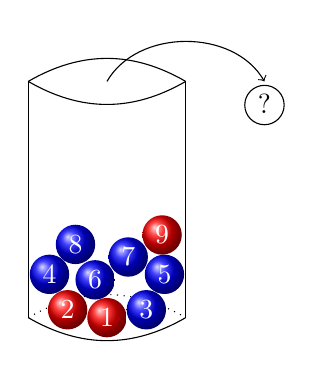
\begin{tikzpicture}
		\draw (0,0) -- (0,-3);
		\draw (2,0) -- (2,-3);
		\draw (0,-3) to [bend right] (2,-3);
		\draw[dotted] (0,-3) to [bend left] (2,-3);
		\draw (0,0) to [bend right] (2,0);
		\draw (0,0) to [bend left] (2,0);
		
		\begin{scriptsize}
		\shade [ball color=red] (1,-3) circle (0.25cm);
		\shade [ball color=red] (0.5,-2.9) circle (0.25cm);
		\shade [ball color=blue] (1.5,-2.9) circle (0.25cm);
		\shade [ball color=blue] (0.27,-2.45) circle (0.25cm);
		\shade [ball color=blue] (1.73,-2.45) circle (0.25cm);
		\shade [ball color=blue] (0.85,-2.52) circle (0.25cm);
		\shade [ball color=blue] (1.27,-2.23) circle (0.25cm);
		\shade [ball color=blue] (0.6,-2.07) circle (0.25cm);
		\shade [ball color=red] (1.7,-1.95) circle (0.25cm);
		\end{scriptsize}
		\node[white] at (1,-3) (1) {1};
		\node[white] at (0.5,-2.9) (2) {2};
		\node[white] at (1.5,-2.9) (3) {3};
		\node[white] at (0.27,-2.45) (4) {4};
		\node[white] at (1.73,-2.45) (5) {5};
		\node[white] at (0.85,-2.52) (6) {6};
		\node[white] at (1.27,-2.23) (7) {7};
		\node[white] at (0.6,-2.07) (8) {8};
		\node[white] at (1.7,-1.95) (9) {9};
		
		\draw[->] (1,0) to [bend left=60] (3,0);
		\draw (3,-0.3) circle (0.25cm);
		\node at (3,-0.29) (a) {?};
	\end{tikzpicture}
\end{document}
%	\caption{Verteilung zu \propref{2_2_6}} 
	%TODO fix caption?
    \includegraphics{../../Material/urne_mit_kugeln.pdf}
\end{center}

\subsection{Urnenmodell mit Zurücklegen: Multinomial-Verteilung}

Gegeben: Urne mit $N$ Kugeln, verschiedenfarbig mit Farben aus $E$, $\abs{E} \ge 2$ 

Ziehe: $n$ Stichproben/Kugeln, wobei nach jedem Zug die Kugel wieder zurückgelegt wird. Uns interessiert die Farbe in jedem Zug, setze also
\begin{align}
	\Omega = E^n \und \sigF = \pows(\Omega) \notag
\end{align}
Zur Bestimmung einer geeigneten Wahrscheinlichkeitsmaßes, nummerieren wir die Kugeln mit $1,\dots, N$, so dass alle Kugeln der Farbe $a \in E$ eine Nummer aus $F_{a} \subset \set{1,\dots, N}$ tragen. Würden wir die Nummern notieren, so wäre
\begin{align}
	\overline{\Omega} = \set{1,\dots, N}^n \und \overline{\sigF} = \pows(\overline{\Omega})\notag
\end{align}
und wir könnten die Gleichverteilung $\overline{\probp} = \Gleich(\overline{\Omega})$ als Wahrscheinlichkeitsmaß für einem einzelnen Zug verwenden. Für den Übergang zu $\Omega$ konstruieren wir  Zufallsvariablen. Die Farbe im $i$-ten Zug wird beschrieben durch
\begin{align}
	X_i: \overline{\Omega} \to E \mit \overline{\omega} = \left( \overline{\omega}_1, \dots, \overline{\omega}_n \right) \mapsto a \text{ falls } \overline{\omega}_i \in F_a\notag
\end{align}
Der Zufallsvektor
\begin{align}
	X = (X_1, \dots, X_n): \overline{\Omega} \to \Omega\notag
\end{align}
beschreibt dann die Abfolge der Farben. Für jedes $\omega \in \Omega$ gilt dann
\begin{align}
	\set{X = \omega} = F_{\omega_1} \times \cdots \times F_{\omega_n} = \bigtimes_{i=1}^{n} F_{\omega_i}\notag
\end{align}
und damit
\begin{align}
	\probp(\set{\omega}) 
	&= \overline{\probp}(X^{-1}(\set{\omega})) = \probp(X=\omega)\notag\\
	&= \frac{\abs{F_{\omega_1}} \cdots \abs{F_{\omega_n}}}{\abs{\overline{\Omega}}}\notag\\
	&= \prod_{i=1}^{n} \frac{\abs{F_{\omega_i}}}{N} =: \prod_{i=1}^{n} \rho(\omega_i)\notag
\end{align}
Zähldichten, die sich als Produkt von Zähldichten schreiben lassen, werden auch als \begriff{Produktdichten} bezeichnet ($\nearrow$  \S 3 Unabhängigkeit). %TODO ref?!?!?!

Sehr oft interessiert bei einem Urnenexperiment nicht die Reihenfolge der gezogenen Farben, sondern nur die Anzahl der Kugeln in Farbe $a \in E$ nach $n$ Zügen. Dies enspricht
\begin{align}
	 \hat{\Omega} 
	 = \set{k = (k_a)_{a \in E} \in \N_{0}^{\abs{E}} \colon \sum_{a \in E} k_a = n}
	 \und \hat{\sigF} = \pows\brackets{\hat{\Omega}}\notag
\end{align}
Den Übergang $\Omega \to \hat{\Omega}$ beschreiben wir durch die Zufallsvariablen
\begin{align}
	Y_a(\omega): \Omega \to \N_{0} \mit \omega = (\omega_1,\dots, \omega_n)\mapsto \sum_{a \in E} \indi_{\set{a}}(\omega_i)\notag
\end{align}
und
\begin{align}
	Y = \brackets{Y_a}_{a\in E}: \Omega \to \hat{\Omega} = \set{k = (k_a)_{a\in E}\colon \sum_{a \in E} k_a = n}\notag
\end{align}

% % % % % % % % % % % % % % % % % % % % 4th lecture % % % % % % % % % % % % % % % % % % % % % % %

Wir erhalten
\begin{align}
	\probp_{Y = k} &= \probp(Y_a = k_a, \quad a \in E)\notag\\
	&= \sum_{\omega \in \Omega:Y(\omega) = k} \prod_{i=1}^{n} \rho(w)\notag\\
	&= \sum_{\omega \in \Omega:Y(\omega) = k} \prod_{a \in E} \rho(\omega) = \begin{bmatrix}
	n \\
	(k)_{a\in E}
	\end{bmatrix}
	\prod_{a \in E} \rho(a)^{k_a}\notag
\end{align}
wobei
\begin{align}
	\binom{n}{k_1, \dots, k_l} = \begin{cases}
	\frac{n!}{k_1 ! k_2 ! \cdots k_l !} & \sum_{i=1}^{l} k_i = n\\
	0 & \sonst
	\end{cases}\notag
\end{align}
der \begriff{Multinomialkoeffizient} welcher die Anzahl der Möglichkeiten beschreibt, $n$ Objekte in $l$ Gruppen aufzuteilen, so dass Gruppe $i$ gerade $k_i$ Objekte beinhaltet.

\begin{definition}
	Sei $l > 2, p = (p_1, \dots, p_l)$ eine Zähldichte und $n \in \N$, dann heißt die Verteilung auf \\
	$\set{k = (k_i)_{i=1,\dots,l} \in \N_{0}^{l} : \sum_{i=1}^{l} k_i = n}$ mit Zähldichte
	\begin{align}
		m((k_1,\dots,k_l)) = \binom{n}{k_1, \dots, k_l}\prod_{i=1}^{l} p_i^{k_i}\notag
%		\end{bmatrix}
	\end{align}
	\begriff{Multinomialverteilung mit Parametern $n$ und $p$}. Wir schreiben auch $\Multi(n,p)$.
\end{definition}

\begin{example}
	Eine Urne enthalte nur schwarze $1$ und weiße $0$ Kugeln $E=\set{0,1}$ und es sei $\rho(1) = 1$ gerade die Proportion der schwarzen Kugeln (= Wahrscheinlichkeit bei einem Zug schwarze zu ziehen), dann ist Wahrscheinlichkeit in $n$ Zügen $k$-mal schwarz zu ziehen:
	\begin{align}
		\binom{n}{k}\prod_{i=0,1} \rho(\omega)^{k_i} = \binom{n}{k}p^k(1-p)^{n-k}.\notag
	\end{align}
	Ein solches (wiederholtes) Experiment mit nur zwei möglichen Ereignissen wird fester Wheit $p = [0,1]$ für eines der Ergebnisse nennen wir auch \begriff{(wiederholtes) Bernoulliexperiment}.
\end{example}

\begin{definition}
	Sei $p \in [0,1]$ un $n \in \N$, dann heißt die Verteilung mit Zähldichte
	\begin{align}
		\rho(k) = \binom{n}{k}p^k (1-p)^{n-k} \mit k \in \set{0,1,\dots,n}.\notag
	\end{align}
	\begriff{Binomialverteilung auf $\set{0, \dots,n}$ mit Parameter $p$} (auch\begriff{Erfolgswahrscheinlichkeit}). Wir schreiben auch $\Bin(n,p)$. Im Fall $n = 1$ nennen wir die Verteilung mit Zähldichte
	\begin{align}
		\rho(0) = 1-p \und \rho(1) = p\notag
	\end{align}
	auch \begriff{Bernoulliverteilung mit Parameter $p$} und schreiben $\Ber(p)$.
\end{definition}
\underline{Urnenmodell ohne Zurücklegen}: \begriff{Hypergeometrische Verteilung}\\
Gegeben: Urne mit $N$ Kugeln verschiedener Farben aus $E$,
\begin{align}
	\abs{E} \ge 2.\notag
\end{align}
Es werden $n \le N$ Stichproben entnommen, wobei die gezogenen Kugeln werde \emph{nicht} in die Urne zurückgelegt.
\begin{example}
	Eine Urne enthalte $S$ schwarze ``$1$'' und $W$ weiße Kugeln ``$0$'' Kugeln, $(E = \set{0,1}, S + W =N)$. Dann ist die Wahrscheinlichkeit in $n$ Zügen ohne Zurücklegen gerade $s$ schwarze und $w$ weiße Kugeln zu ziehen
	\begin{align}
		\rho(w) = \frac{\binom{W}{w}\binom{S}{s}}{\binom{N}{n}} \mit 0 \le s \le S,\; 0 \le w \le W,\; s+w = n,\; S+W = N.\notag
	\end{align}
\end{example}

\begin{proof}
	Hausaufgabe! %TODO add nummer later
\end{proof}

\begin{definition}
	Seinen $N \in \N, W \le N, n \in \N$, dann heißt die Verteilung auf $\set{0,\dots,n}$ mit Zähldichte
	\begin{align}
		\rho(w) = \frac{\binom{wW}{w}\binom{N-W}{n-w}}{\binom{N}{n}} \mit w = \max\set{0,n=N+W}, \dots, \min\set{W,n},\notag
	\end{align}
	die \begriff{Hypergeometrische Verteilung} mit Parametern $N,W,n$. Wir schreiben $\Hyper(N,W,n)$.
\end{definition}

\section{\person{Poisson}-Approximation un \person{Poisson}-Verteilung}

$\Bin(n,p)$ ist zwar explizit und elementar definiert, jedoch für große $n$ mühsam auszuwerten. Für seltene Ereignisse $(n \text{ groß},p \text{ klein})$ verwende daher:

\begin{proposition}[Poisson-Approximation]
	Sei $\lambda$ und $(p_n)_{n\in\N}$ eine Folge in $[0,1]$ mit
	\begin{align}
		np_n \to \lambda,\quad n \to \infty.\notag
	\end{align}
	Dann gilt $\forall k \in \N$ für die Zähldichte der $\Bin(n,p_n)$-Verteilung
	\begin{align}
		\lim_{n \to \infty} \binom{n}{k}p_n^k(1-p)^{n-k} = e^{-\lambda} \frac{\lambda^k}{k!}.\notag
	\end{align}
\end{proposition}
\begin{proof}
	Sei $k \in \N_{0}$ fix, dann
	\begin{align} %TODO fix alignment and now there are tags, but \notag is added?!
		\binom{n}{k} = \frac{n!}{k!(n-k)!} &= \frac{n^k}{k!}\frac{n(n-1)\cdots(n-k+1)}{n^k}\notag\\
		&= \frac{n^k}{k!}\cdot 1 (1-\frac{1}{n}\cdots \frac{1}{\frac{k-1}{n}})\notag\\
		&\overset{n \to \infty}{~} \frac{n^k}{k!},\notag
	\end{align}
	wobei $a(l) \overset{n \to \infty}{\sim} b(l) \Leftrightarrow \frac{a(l)}{b(l)} \xrightarrow{n\to \infty} 1$. Damit
	\begin{align}%TODO fix alignment
		\binom{n}{k}p_n^k (1-p)^{n-k} &\overset{n \to \infty}{\sim} \frac{n^k}{k!}p_n^k(1-p_n)^{n-k}\notag\\
		&\overset{n \to \infty}{\sim} \frac{\lambda^k}{k!}(1-p_n)^n\notag\\
		&=\frac{\lambda^n}{k!}\brackets{1 - \frac{np_n}{n}}^n\notag\\
		&\xrightarrow{n \to \infty} \frac{\lambda^n}{k!}e^{-\lambda}.\notag
	\end{align}
\end{proof}
Der erhaltene Grenzwert liefert die Zähldichte auf $\N_{0}$, denn 
\begin{align}
	\sum_{k=0}^{\infty}\frac{\lambda^k}{k!}e^{-\lambda} = e^{-\lambda}\sum_{k=0}^{\infty}\frac{\lambda^{k}}{k!} = e^{-\lambda}e^{\lambda} = 1\notag
\end{align}
\begin{definition}
	Sei $\lambda >0$. Dann heißt das auf $(\N_{0}, \probp(\N_{0}))$ definiert Wahrscheinlichkeitsmaß mit
	\begin{align}
		\probp(\set{k}) = \frac{\lambda^k}{k!}e^{-\lambda} \quad k \in \N_{0},\notag
	\end{align}
	\begriff{Poissonverteilung mit Parameter $\lambda$}. Schreibe $\Pois(\lambda)$.
\end{definition}
Die Poissonverteilung ist ein natürliches Modell für die Anzahl von zufälligen, seltenen Ereignissen (z.B. Tore im Fußballspiel, Schadensfälle einer Versicherung, ...).
% Bedingte Wahrscheinlichkeiten und (Un)-abbhängigkeit}
\chapter[Bedingte Wahrscheinlichkeiten und (Un)-abbhängigkeit]{Bedingte Wkeiten und (Un)-abbhängigkeit}
\chaptermark{Bedingte Wheiten und (Un)-abbhängigkeit}

\section{Bedingte Wahrscheinlichkeiten}
\begin{example}
	\proplbl{3_1_1}
	Das Würfeln mit zwei fairen, sechsseitigen Würfeln können wir mit 
	\begin{align}
		\Omega = \set{(i,j,), i,j \in \set{1,\dots,6}}\notag
	\end{align}
	und $\probp = \Gleich(\Omega)$. Da $\abs{\Omega} = 36$ gilt also
	\begin{align}
		\probp(\set{\omega}) = \frac{1}{36} \quad \forall \omega \in \Omega.\notag
	\end{align}
	Betrachte das Ereignis
	\begin{align}
		A = \set{(i,j) \in \Omega : i + j = 8},\notag
	\end{align}
	dann folgt
	\begin{align}
		\probp(A) = \frac{5}{36}.\notag
	\end{align}
	Werden die beiden Würfel nach einander ausgeführt, so kann nach dem ersten Wurf eine Neubewertung der Wahrscheinlichkeit von $A$ erfolgen.\\
	Ist z.B.:
	\begin{align}
		B = \set{(i,j) \in \Omega, i = 4}\notag
	\end{align}
	eingetreten, so kann die Summe 8 nur durch eine weitere 4 realisiert werden, also mit Wahrscheinlichkeit
	\begin{align}
		\frac{1}{6} = \frac{\abs{A \cap B}}{\abs{B}}.\notag 
	\end{align}
	Das Eintreten von $B$ führt also dazu, dass das Wahrscheinlichkeitsmaß $\probp$ durch ein neues Wahrscheinlichkeitsmaß $\probp_{B}$ ersetzt werden muss. Hierbei sollte gelten:
	\begin{align}
		 &\text{Renormierung: }\probp_{B} = 1\label{Renorm}\tag{R}\\
		 &\text{Proportionalität: Für alle} A \subset \sigF \mit A \subseteq B \text{ gilt }
		 \probp_{B}(A) = c_B \probp(A) \text{ mit einer Konstante } c_B.\label{Prop}\tag{P}
    \end{align}
\end{example}

\begin{lemma}
	Sei $(\Omega, \sigF, \probp)$ Wahrscheinlichkeitsraum und $B \in \sigF$ mit $\probp(B) > 0$. Dann gibt es genau ein Wahrscheinlichkeitsmaß $\probp_B$ auf $(\Omega, \sigF)$ mit den Eigenschaften \eqref{Renorm} und \eqref{Prop}. Dieses ist gegeben durch
	\begin{align}
		\probp_{B}(A) = \frac{\probp(A\cap B)}{\probp(B)} \quad \forall A \in \sigF.\notag
	\end{align}
\end{lemma}

\begin{proof}
	Offenbar erfüllt $\probp_{B}$ wie definiert \eqref{Renorm} und \eqref{Prop}. Umgekehrt erfüllt $\probp_{B}$ \eqref{Renorm} und \eqref{Prop}. Dann folgt für $A \in \sigF$:
	\begin{align}
		\probp_{B}(A) = \probp_{B}(A\cap B) + \underbrace{\probp_{B}(A\setminus B)}_{= 0, \text{ wegen } \eqref{Renorm}} \overset{\eqref{Prop}}{=} c_B \probp(A \cap B).\notag
	\end{align}
	Für $A=B$ folgt zudem aus \eqref{Renorm}
	\begin{align}
		1 = \probp_{B}(B) = c_B \probp(B)\notag
	\end{align}
	also $c_B = \probp(B)^{-1}$.
\end{proof}

% % % % % % % % % % % % % % % % % % % % % % % % % % % 5th lecture % % % % % % % % % % % % % % % % % % % % % % % % % % %

\begin{definition}
	\proplbl{3_1_3}
	Sei $(\Omega, \sigF, \probp)$ Wahrscheinlichkeitsraum und $B \in \sigF$ mit $\probp(B) > 0$. Dann heißt
	\begin{align*}
		\probp(A\vert B) := \frac{\probp(A\cap B)}{\probp(B)} \mit A\in \sigF
	\end{align*}
	die \begriff{bedingte Wheit von $A$ gegeben $B$}.
	Falls $\probp(B) = 0$, setze
	\begin{align*}
		\probp(A \vert B) = 0 \mit \forall A \in \sigF
	\end{align*}
\end{definition}

\begin{example} %TODO ref
	In der Situation \propref{3_1_1} gilt % 
	\begin{align*}
	A \cap B = \set{(4,4)}
	\intertext{und damit}
	\probp(A \vert B) = \frac{\probp(A\cap B)}{\probp(B)} = \frac{\frac{1}{36}}{\frac{1}{6}} = \frac{1}{6}
	\end{align*}
\end{example}
Aus \propref{3_1_3} ergibt sich
\begin{lemma}[Multiplikationsformel]
	\proplbl{3_1_4}
	Sei $(\Omega, \sigF, \probp)$ Wahrscheinlichkeitsraum und $A_1, \dots, A_n \in \sigF$. Dann
	\begin{align*}
		\probp(A_1 \cap \cdots \cap A_n) = \probp(A_1)\probp(A_2 \vert A_n) \dots \probp(A_n \vert A_1 \cap \cdots \cap A_{n-1})
	\end{align*}
\end{lemma}

\begin{proof}
	Ist $\probp(A_1 \cap \dots \cap A_n) = 0$, so gilt auch $\probp(A_n \vert \bigcap_{i=1}^{n-1}) = 0$. Andernfalls sind alle Faktoren der rechten Seite ungleich 0 und
	\begin{align*}
		\probp(A_1)\probp(A_2 \vert A_1) \dots \probp(A_n \vert \bigcap_{i=1}^{n-1} A_i) \\
		= \probp(A_1) \cdot \frac{\probp(A_1 \cap A_2)}{\probp(A_1)} \dots \frac{\probp(\bigcap_{i=1}^{n} A_i)}{\probp(\bigcap_{i=1}^{n-1}A_i)} = \probp(\bigcap_{i=1}^n A_i)	
	\end{align*}
\end{proof} %TODO add ref.
Stehen die $A_i$ in \propref{3_1_4} in einer (zeitlichen) Abfolge, so liefert Formel einen Hinweis, wie Wahrscheinlichkeitsmaße für \begriff{Stufenexperimente} konstruiert werden können. Ein \emph{Stufenexperiment} aus $n$ nacheinander ausgeführten Teilexperimenten lässt sich als \begriff{Baumdiagramm} darstellen.

%TODO Baumdiagramm
%\begin{tikzpicture}
%	%TODO
%\end{tikzpicture}

\begin{proposition}[Konstruktion des Wahrscheinlichkeitsmaßes eines Stufenexperiments]
	\proplbl{3_1_6}
	Gegeben seinen $n$ Ergebnisräume $\Omega_i = \set{\omega_i (1), \dots, \omega_i (k)}, k \in \N \cup \set{\infty}$ und es sei $\Omega = \bigtimes_{i = 1}^n \Omega_i$ der zugehörige Produktraum. Weiter seinen $\sigF_i$ $\sigma$-Algebren auf $\Omega_i$ und $\sigF = \bigotimes_{i=1}^n \sigF_i$ die Produkt-$\sigma$-Algebra auf $\Omega$. Setze $\omega = (\omega_1,\dots,\omega_n)$ und
	\begin{align*}
		[\omega_1,\dots,\omega_n]:= \set{\omega_1}\times \dots \times \set{\omega_n} \times \Omega_{m-1} \times \Omega_{n},\quad m\le n\\
		\probp(\set{\omega_m}[\omega_1,\dots,\omega_{m-1}])
	\end{align*} %TODO check indices, m-1 instead of m+1?
	für die Wheit in der $m$-ten Stufe des Experiments $\omega_m$ zu beobachten, falls in den vorausgehenden Stufen $\omega_1,\dots,\omega_{m-1}$ beobachten wurden. Dann definiert
	\begin{align*}
		\probp(\set{\omega}) := \probp(\set{\omega_1})\prod_{m=2}^{n}\probp\brackets{\set{\omega_m} \mid [\omega_1, \dots, \omega_{m-1}]}
		%TODO maybe wrong here. check
	\end{align*}
	ein Wahrscheinlichkeitsmaß auf $(\Omega, \sigF, \probp)$.
\end{proposition}

\begin{example}[\person{Polya}-Urne]
	Gegeben sei eine Urne mit $s$ Schwarze und $w$ weiße Kugeln. Bei jedem Zug wird die  gezogene Kugel zusammen mit $c\in \N_0\cup \set{-1}$ weiteren Kugeln derselben Farbe zurückgelegt.
	\begin{itemize} %TODO seen both in chapter 2.2, but big bracket behind.
		\item $c=0$: Urnenmodell mit Zurücklegen
		\item $c=-1$: Urnenmodell ohne Zurücklegen
	\end{itemize}
	Beide schon in Kapitel 2.2 gesehen.\\
	Sei $c\in \N$. (Modell für zwei konkurrierende Populationen) Ziehen wir $n$-mal, so erhalten wir ein $n$-Stufenexperiment mit 
	\begin{align*}
		\Omega = \set{0,1}^n \mit \text{ 0 = ``weiß'', 1 = ``schwarz''}\mit	(\Omega_i = \set{0,1})
		\intertext{Zudem gelten im ersten Schritt}
		\probp(\set{0}) = \frac{w}{s+w} \und \probp(\set{1}) = \frac{s}{w+s}
		\intertext{sowie}
		\probp(\set{\omega_m} \mid [\omega_1, \dots \omega_{m-1}]) = 
		\begin{cases} %TODO fix brackets!
		\frac{w+c(m-1 - \sum_{i=1}^{m-1}\omega_i)}{s+w+c(m-1)} & \omega_m = 0\\
		\frac{s + c\sum_{i=1}^{m-1}\omega_i}{s+w+c(m-1)} & \omega_m = 1
		\end{cases}
	\end{align*}
	Mit \propref{3_1_6} folgt als Wahrscheinlichkeitsmaß auf $(\Omega, \pows(\Omega))$
	\begin{align*}
		\probp(\set{(\omega_1, \dots, \omega_n)}) &= \probp(\set{\omega_1})\prod_{m=2}^n \probp(\set{\omega_m}\mid [\omega_1,\dots,\omega_{m-1}])\\
		&=\frac{\prod_{i=0}^{l-1}(s+c_i)\prod_{i=0}^{n-l-1}}{\prod_{i=0}^n (s+w+c_i)} \mit l=\sum_{i=1}^n \omega_i.
		\intertext{Definiere wir nun die Zufallsvariable}
		S_n:\Omega &\to \N_0 \mit (\omega_1, \dots, \omega_n) \mapsto \sum_{i=1}^n \omega_i
		\intertext{welche die Anzahl der gezogenen schwarzen Kugeln modelliert, so folgt,}
		\probp(S_n = l) &= \binom{n}{l}\frac{\prod_{i=0}^{l-1}(s+c_i) \prod_{j=0}^{n-l-1}(\omega + c_j)}{\prod_{i=0}^n(s+w+c_i)}
		\intertext{Mittels $a:= \sfrac{s}{c},b:= \sfrac{w}{c}$ folgt}
		\probp(S_n = l) &= \frac{\prod_{i=0}^{l-1}(-a-i)\prod_{i=0}^{-b-j-1}}{\prod_{i=0}^n (-a-b-i)} = \frac{\binom{-a}{l}\binom{-b}{n-l}}{\binom{-a-b}{n}}\\ &\mit l \in \set{0,\dots,n} 
	\end{align*}
	Dies ist die \begriff{\person{Polya}-Urne} auf $\set{0,\dots,n}, n \in \N$ mit Parametern $a,b > 0$.
\end{example}

\begin{example}
	Ein Student beantwortet eine Multiple-Choice-Frage mit 4 Antwortmöglichkeiten, eine davon ist richtig. Er kennt die richtige Antwort mit Wheit $\sfrac{1}{3}$. Wenn er diese kennt, so wählt er diese aus. Andernfalls wählt er zufällig (gleichverteilt) eine Antwort.\\
	Betrachte
	\begin{align*}
		W = \set{\text{richtige Antwort gewusst}}\\
		R = \set{\text{Richtige Antwort gewählt}}
		\intertext{Dann}
		\probp(W) = \frac{2}{3}, \probp(R \vert W) = 1, \probp(R \vert W^C) = \frac{1}{4} 
	\end{align*}
	Angenommen, der Student gibt die richtige Antwort. Mit welcher Wahrscheinlichkeit hat er diese gewusst?
	\begin{align*}
		\probp(W\vert R) = \text{ ?}
	\end{align*}
\end{example}

\begin{proposition}
	\proplbl{3_1_9}
	Sei $(\Omega, \sigF, \probp)$ Wahrscheinlichkeitsraum und $\Omega = \bigcup_{i \in I} B_i$ eine höchstens abzählbare Zerlegung in paarweise disjunkte Ereignisse $B_i \in \sigF$.
	\begin{enumerate} %TODO set itemize references. or use enumerate?
		\item \emph{Satz von der totalen Wahrscheinlichkeit:} Für alle $A \in \sigF$
		\begin{align*}
			\probp(A) = \sum_{i\in I} \probp(A\vert B_i)\probp(B_i) \label{eq:totWkeit}\tag{totale Wahrscheinlichkeit}
		\end{align*} 
		\item \emph{Satz von \person{Bayes}:} Für alle $A \in \sigF$ mit $\probp(A) > 0$ und alle $h \in I$
		\begin{align*}
			\probp(B_h \vert A) = \frac{\probp(A \vert B_h)\probp(B_h)}{\sum_{i\in I}\probp(A\vert B_i)\probp(B_i)} \label{eq:bayes}\tag{Bayes}
		\end{align*}
	\end{enumerate}
\end{proposition}

\begin{proof}
	\begin{enumerate}
		\item Es gilt:
		\begin{align*}
			\sum_{i\in I} \probp(A\vert B_i)\probp(B_i) \defeq \sum_{i\in I}\frac{\probp(A \cap B_i)}{\probp(B_i)}\probp(B_i) = \sum_{i\in I} \probp(A \cap B_i) \overset{\sigma-add.}{=} \probp(A)
		\end{align*}
		\item 
		\begin{align*}
			\probp(B_h \vert A) \defeq \frac{\probp(A \cap B_h)}{\probp(A)} \defeq \frac{\probp(A \vert B_h)\probp(B_h)}{\probp(A)}
		\end{align*}
		also mit a) auch b). %TODO add refs
	\end{enumerate}
\end{proof}

\begin{example}
	In der Situation von \propref{3_1_3} folgt mit dem \propref{3_1_9} \eqref{eq:totWkeit} der totalen Wahrscheinlichkeit
	\begin{align*}
		\probp(R) &= \probp(R \vert W)\probp(W) + \probp(R\vert W^C)\probp(W^C)\\
		&= 1\cdot \frac{2}{3} + \frac{1}{4}\frac{1}{3} = \frac{3}{4}
		\intertext{und mit dem \propref{3_1_9} \eqref{eq:bayes}} %Bayes
		\probp(W \vert R) &= \frac{\probp(R \vert W)\probp(W)}{\probp(R)} = \frac{1\frac{2}{3}}{\frac{3}{4}} = \frac{8}{9} \text{ für die gesuchte Wahrscheinlichkeit.}
	\end{align*} %TODO
%	\begin{tikzpicture}
%		
%	\end{tikzpicture} 
\end{example}
% trees in Latex?
% https://tex.stackexchange.com/questions/5447/how-can-i-draw-simple-trees-in-latex/5451
\section{(Un)-abhängigkeit} \label{sec_unabhangigkeit}
In vielen Fällen besagt die Intuition über verschiedene Zufallsexperimente/ Ereignisse, dass diese sich \emph{nicht} gegenseitig beeinflussen. Für solche $A,B \in \F$ mit $\probp(A) > 0, \probp(B) > 0$ sollte gelten
\begin{align*}
	\probp(A\mid B) = \probp(B), \quad \probp(B\mid A) = \probp(B).
\end{align*}
\begin{definition}[(stochastisch)unabhängig]
	\proplbl{3_2_11}
	$(\Omega, \F, \probp)$ WRaum. Zwei Ereignisse $A,B \in \F$ heißt \begriff{(stochastisch) unabhängig bezüglich $\probp$}, falls
	\begin{align*}
		\probp(A\cap B) = \probp(A)\probp(B)
	\end{align*}
	Wir schreiben auch $A B$.
\end{definition}
\begin{example}
	Würfeln mit 2 fairen, sechsseitigen Würfel:
	\begin{align*}
		\Omega = \set{(i,j) \mid i,j \in\set{1,\dots,n}},\quad \F = \pows(\Omega), \quad \probp = \Gleich(\Omega)
	\intertext{Betrachte}
		A:= \set{(i,j) \in \Omega, i \text{ gerade}}\\
		B:= \set{(i,j) \in \Omega, j > 2}
	\end{align*}
	In diesem Fall, erwarten wir intuitiv Unabhängigkeit von $A$ und $B$.\\
	In der Tat % start using \P instead of \probp!
	\begin{align*}
		\P(A) = \frac{1}{2}, \quad \P(B) = \frac{1}{3} \mit \P(A\cap B) = \frac{1}{6}
		\intertext{erfüllt}
		\P(A\cap B) = \P(A)\P(B).
	\end{align*}
	Betrachte nun
	\begin{align*}
		C:= \set{(i,j) \in \Omega, i\neq j = 1}\\
		D:= \set{(i,j) \in \Omega, i = 6}
		\intertext{dann gilt}
		\P(C) = \frac{1}{6}, \quad \P(D) = \frac{1}{6}
		\intertext{und wegen $C \cap D = \set{(6,1)}$ folgt}
		\P(C\cap D) = \frac{1}{36} = \frac{1}{6} \frac{1}{6} = \P(C \setminus D)
	\end{align*}
	$C$ und $D$ sind also \emph{stochastisch} unabhängig, obwohl eine kausale Abhängigkeit vorliegt!
\end{example}
\begin{definition}[unabhängig bezüglich $\P$]
	$(\Omega, \F, \P)$ WRaum und $I \neq \emptyset$ endliche Indexmenge. Dann heißt die Familie $(A_i)_{i \in I}$ von Ereignissen in $\F$ \begriff{unabhängig bezüglich $\P$}, falls für alle $J \subseteq I, J \neq \emptyset$ gilt:
	\begin{align*}
		\P\brackets{\bigcap_{i\in J}A_i} = \prod_{i\in J} \P(A_i)
	\end{align*}
	Offensichtlich impliziert die Unabhängigkeit einer Familie die paarweise Unabhängigkeit je zweier Familienmitglieder nach \propref{3_2_11}. Umgekehrt gilt dies nicht!
\end{definition}
\begin{example}[Abhängigkeit trotz paarweiser Unabhängigkeit]
	Betrachte 2-faches Bernoulliexperiment mit Erfolgswahrscheinlichkeit $\sfrac{1}{2}$, d.h.
	\begin{align*}
		\Omega = \set{0,1}^2, \quad \F = \pows(\Omega), \quad \P = \Gleich(\Omega)
		\intertext{sowie}
		A = \set{1}\times \set{0,1} \qquad \text{(Münzwurf: erster Wurf Zahl)}\\
		B = \set{0,1}\times \set{1} \qquad \text{(Münzwurf: zweiter Wurf Zahl)}\\
		C = \set{0,0}\times \set{1,1} \qquad \text{(beide Würfe selbes Ergebnis)}
	\end{align*}
	Dann gelten
	\begin{align*}
		\P(A) = \frac{1}{2} = \P(A) = \P(B)
		\intertext{und}
		\P(A\cap B) = \P(\set{(1,1)}) = \frac{1}{4} = \P(A)\P(B)\\
		\P(A\cap C) = \P(\set{(1,1)}) = \frac{1}{4} = \P(A)\P(C)\\
		\P(B\cap C) = \P(\set{(1,1)}) = \frac{1}{4} = \P(B)\P(C)
	\end{align*}
	also paarweise Unabhängigkeit.\\
	Aber
	\begin{align*}
		\P(A\cap B \cap C) = \P(\set{(1,1)}) = \frac{1}{4} + \P(A)\P(B)\P(C)
		\intertext{und $A,B,C$ sind \emph{nicht} stochastisch unabhängig.}
	\end{align*}
\end{example}
\begin{definition}[Unabhängige Messräume]
	\proplbl{3_2_15}
	% started using \O for \Omega and \E for this special generating set E_i
	$(\O, \F,\P)$ Wahrscheinlichkeitsraum, $I \neq \emptyset$ Indexmenge und $(E_i, \E_i)$ Messräume
	\begin{enumerate}
		\item Die Familie $\F_i \subset \F, i \in I$, heißen \emph{unabhängig}, wenn für die $J \subseteq I, I \neq \emptyset, \abs{J} < \infty$ gilt
		\begin{align*}
			\P\brackets{\bigcap_{i=1} A_i} = \prod_{i\in J} \P(A_i) \qquad \text{ für beliebige } A_i \in \F_i, i \in J
		\end{align*}
		\item Die Zufallsvariable $X_i: (\O, \F) \to (E_i, \E_i), i \in I$, heißen \emph{unabhängig}, wenn die $\sigma$-Algebren
		\begin{align*}
			\sigma(X_i) = X^{-1}(\E_i) = \set{\set{X_i \in F}, F \in \E_i}, \quad i \in I
		\end{align*}
		unabhängig sind.
	\end{enumerate}
\end{definition}
\begin{lemma}[Zusammenhang der Definitionen]
	\proplbl{3_2_16}
	$(\O,\F,\P)$ Wahrscheinlichkeitsraum, $I \neq \emptyset, A \in \F, i \in I$.\\
	Die folgenden Aussagen sind äquivalent:
	\begin{enumerate}
		\item Die Ereignisse $A_i, i \in I$ sind unabhängig. 
		\item Die $\sigma$-Algebren $\sigma(A_i), i \in I$ sind unabhängig.
		\item Die Zufallsvariablen $\indi_{A_i}, i \in I$ sind unabhängig.
	\end{enumerate}
\end{lemma}
\begin{proof} %TODO add ref?
	Da die Unabhängigkeit über endliche Teilemengen definiert ist, können wir oBdA $I = \set{1, \dots, n}$ annehmen. 
	\begin{itemize}
		\item Da $\sigma(\indi_{A_i}) = \sigma(A_i)$ folgt die Äquivalenz von 2. und 3. direkt aus \propref{3_2_15}.
		\item Zudem ist 2. $\to $ 1. klar!
		\item Für 1 $\to$ 2. genügt es zu zeigen, dass
			\begin{align*}
				A_1, \dots, A_n \text{ unabhängig } &\Rightarrow B_1, \dots, B_n \text{ unabhängig von } B_i \in \set{\emptyset, A_i, A_i^C, \O}.
				\intertext{Rekursive folgt dies bereits aus}
				A_1,\dots, A_n \text{ unabhängig } &\Rightarrow B_1, A_2, \dots, A_n \text{ unabhängig mit } B_1 \in \set{\emptyset, A_1, A_1^C, \O}.
			\end{align*}
		Für $B_1 \in \set{\emptyset, A_1, \O}$ ist dies klar.\\
		Sei also $B_1 = A_1^C$ und $J \subseteq I, J \neq \emptyset$. Falls $1 \not \in J$, ist nichts zu zeigen. Sei $1 \in J$, dann gilt mit
			\begin{align*}
				A &= \bigcap_{i\in J, i \neq 1} A_i
				\intertext{sicherlich}
				\P\brackets{A_1^C \cap A} &= \P(A \setminus (A_1 \cap A))\\
				&= \P(A) - \P(A_1 \cap A)\\
				&= \prod_{i\in J\setminus \set{1}} \P(A_i) - \prod_{i\in J}(A_i)\\
				&= (1- \P(A_1))\prod_{i\in J\setminus \set{1}} \P(A_i)\\
				&= \P\brackets{A_1^C})\prod_{i\in J\setminus \set{1}} \P(A_i)
			\end{align*} 
	\end{itemize}
\end{proof}
Insbesondere zeigt das \propref{3_2_16}, dass wir in einer Familie unabhängiger Ereignisse beliebig viele Ereignisse durch ihr Komplement, $\emptyset$ oder $\O$ ersetzen können, ohne die Unabhängigkeit zu verlieren.
\begin{proposition}
	\proplbl{3_2_17}
	$(\O, \F, \P)$ Wahrscheinlichkeitsraum und $\F_i \subseteq \F, i \in I$, seien $\cap$-stabil Familien von Ereignissen. Dann
	\begin{align*}
		\F_i, i \in I \text{ unabhängig } \Leftrightarrow \sigma(\F_i), i \in I \text{ unabhängig}. 
	\end{align*}
\end{proposition}

\begin{proof}
	OBdA sei $I = \set{1, \dots, n}$ und das $\O \in \F_i, i \in I$.
	\begin{itemize}
		\item $\Leftarrow$: trivial, da $\F_i \subseteq \sigma(\F_i)$ und das Weglassen von Mengen erlaubt ist.
		\item $\Rightarrow$: zeigen wir rekursive
			\begin{enumerate}
				\item Wähle $F_i \in \F_i, i = 2, \dots,n$ und defnieren für $F \in \sigma(\F_i)$ die endlichen Maße
				\begin{align*}
					\mu(F) = \P\brackets{\bigcap_{i=1}^n F_i} \und \nu(F) = \prod_{i=1}^n \P(F_i)
				\end{align*}
				\item Da die Familien $\F_i$ unabhängig sind, gilt
				\begin{align*}
					\mu\mid_{\F_1} = \nu\mid_{\F_1}
				\end{align*}
				Nach Eindeutigkeitssatz für Maße (\proplbl{1_1_19}) folgt $\mu\mid_{\sigma(\F_1)} = \nu\mid_{\sigma(\F_1)}$ also
				\begin{align*}
					\P(\bigcap_{i=1}^n F_i) = \P(F)\P(F_1)\dots \P(F_n)
				\end{align*}
				für alle $F \in \sigma(\F_i)$ und $F_i \in \F_i, i = 1, \dots, n$. Da $\O \in \F_i$ für alle $i$ gilt die erhaltene Produktformel auf für alle Teilemenge $J \subseteq I$.\\
				Also sind
				\begin{align*}
					\sigma(\F_1), \F_2, \dots, \F_n \text{unabhängig}
				\end{align*}
				\item Wiederholtes Anwenden von $1$ und $2$ liefert den \propref{3_2_17}.
			\end{enumerate}
	\end{itemize}
\end{proof}

Mittels \propref{3_2_17} folgen:

\begin{conclusion}
	$(\O,\F,\P)$ Wahrscheinlichkeitsraum und
	\begin{align*}
		\F_{i,j} \subseteq \F, \quad 1 \le \dots \le n, 1 \le j \le m(i)
	\end{align*}
	unabhängige, $\cap$-stabile Familien.
	Dann sind auch
	\begin{align*}
		\G_i = \sigma(\F_{i,1},\dots, \F_{i,m(i)}), \quad 1 \le i \le n
	\end{align*}
	unabhängig.
\end{conclusion}

\begin{conclusion}
	$(\O,\F,\P)$ Wahrscheinlichkeitsraum, und
	\begin{align*}
		X_{ij}: \O \to E, \quad 1 \le i \le n, 1 \le j \le m(i)
	\end{align*}
	unabhängige Zufallsvariablen. Zudem seinen $f_i: E^{m(i)} \to \R$ messbar. Dann sind auch die Zufallsvariablen
	\begin{align*}
		f_i(X_{i1}, \dots, X_{im(i)}), \quad 1 \le i \le n
	\end{align*}
	unabhängig.
\end{conclusion}

\begin{example}
	$X_1, \dots, X_n$ unabhängige reelle Zufallsvariablen. Dann sind auch
	\begin{align*}
		Y_1 = X_1, Y_2 = X_2 + \cdots + X_n
	\end{align*}
	unabhängig.
\end{example}

\chapter{Test}


\part*{Anhang}
\addcontentsline{toc}{part}{Anhang}
\appendix

\nocite{*}
\bibliography{literatur}
\bibliographystyle{acm}

%\printglossary[type=\acronymtype]

\printindex

\end{document}
